\documentclass{article}
\usepackage[frenchb]{babel}
\usepackage[utf8]{inputenc}
\usepackage[T1]{fontenc}
\usepackage{alltt}
\usepackage{minted}
\usepackage{amsmath}
\usepackage{amsfonts}
\usepackage{graphicx}
\usepackage{color}
\usepackage{subfig}
\usepackage{setspace}
\usepackage{verbatim}
\usepackage{url}
\usepackage[hidelinks=true]{hyperref}
\usepackage{caption}

\usepackage{listings}

\definecolor{green_ruby}{rgb}{0.30, 0.62, 0.28}
\definecolor{gray_ruby}{rgb}{0.5,0.5,0.5}
\definecolor{mauve_ruby}{rgb}{0.58,0,0.82}

\lstdefinestyle{RubyStyle}{
  backgroundcolor=\color{white},
  breakatwhitespace=false,
  breaklines=true,              
  captionpos=b,   
  commentstyle=\color{green_ruby},  
  extendedchars=true,     
  frame=single,	
  keepspaces=true,
  language=Ruby,
  keywordstyle=\color{blue},
  numbersep=5pt,
  numberstyle=\tiny\color{gray_ruby},
  rulecolor=\color{black},
  showspaces=false,
  showstringspaces=false,
  showtabs=false,
  stepnumber=2,
  stringstyle=\color{mauve_ruby},
  tabsize=2,
}

\usepackage{fancyhdr}
\pagestyle{fancy}
\renewcommand\headrulewidth{1pt}
\fancyhead[L]{Web2Control}
\fancyhead[R]{Enseirb-Matmeca}


%%%%%%%%%%%%%%%% Variables %%%%%%%%%%%%%%%%
\def\titre{\\Groupe PFA WEB2CONTROL \\ \vspace{5 mm}
Réalisation d'une application démonstrative} }
\def\titregauche{Projet S8}
\def\titredroite{Réalisation du backend}
\def\filiere{informatique}
\def\annee{$2^{\grave{e}me}$}
\def\anneescolaire{2015/2016}
\def\promotion{2017}
\def\equipe{RIFKI Imane\\CHASSAIGNE Théo \\COOK Clément\\DELMON Luc \\ DURAND Antoine\\EL AMRI Mehdi\\PETRO Romain}
\def\encadrant{LOMBARDY Sylvain} 
\def\client{INRIA Mnemosyme}
%%%%%%%%%%%%%%%%%%%%%%%%%%%%%%%%%%%%%%%%%%%

\newcommand{\HRule}{\rule{\linewidth}{0.5mm}}

\begin{document}

\begin{titlepage}

\begin{center}

% Upper part of the page

\includegraphics[width=0.3\textwidth]{enseirb.png}\\[1cm]

\textsc{\LARGE ENSEIRB-MATMECA}\\[1cm]

\textsc{\Large {Filière \filiere, \annee année}}\\[0.5cm]
\textsc{\Large {Promotion \promotion}}\\[0.5cm]
\textbf{\huge Cahier des charges} }
\vspace{5 mm}

% Title
\HRule \\[0.4cm]
{ \huge \bfseries \titre}\\[0.4cm]

\HRule \\[1.5cm]

% Author and supervisor
\begin{minipage}{0.4\textwidth}
\begin{flushleft} \large
\emph{Auteurs :}\\
\equipe
\end{flushleft}
\end{minipage}
\begin{minipage}{0.4\textwidth}
\begin{flushleft} \large
\emph{~~~~~~~~~~~~Encadrant :} \\
\encadrant \\
\emph{\\~~~~~~~~~~~~Clients :} \\ 
\client
\end{flushleft}
\end{minipage}

\vfill

% Bottom of the page
{\large \today}

\end{center}

\end{titlepage}

\tableofcontents

\newpage

\section{Contexte et objectifs généraux}

\subsection{Contexte}

Dans le cadre du projet de fin d’année proposé par l’INRIA, nous avons rédigé sur la période de septembre à décembre une documentation détaillée sur l’utilisation de bibliothèques publiques de machine-learning et sur le fonctionnement des API Twitter et Facebook - plus précisément sur la récolte de données publiques en masse via ces API.

Cette documentation a pour but d’expliquer à un novice du machine-learning comment fonctionnent les algorithmes et les bibliothèques  et comment combiner les fonctions de ces bibliothèques aux API afin de faire du traitement de données sociales en masse sans avoir de grandes connaissances dans le domaine.

Afin d’illustrer notre documentation, nous allons réaliser - toujours dans le cadre de notre PFA et au cours  de la période  de  janvier à mai - une application illustrative basé sur le réseau social Twitter.

Cette application n’a pas pour but d’être commercialisée et sa définition peut encore évoluer au cours du développement.

\subsection{Objectifs généraux}

L’objectif général est de réaliser une application locale connectée développée en python qui utilisera une partie des tweets de Twitter  pour effectuer des regroupements et qui sera en mesure de ranger automatiquement les tweets dans certaines catégories définies à l’avance sur la base de leurs points communs (événements, lieux, sujets), mais également sur la base des comportements autour de ces tweets ( taux de retweet, réactivité des retweeter, taille des conversations sur les tweets). Certains groupements  pourront appartenir à plusieurs catégories.

L’objectif caché est de démontrer l’efficacité de bibliothèques présentées dans notre documentation et d’illustrer leur utilisation sur un cas concret.

\section{Documentation}

Les termes techniques spécifiques employés dans la suite du présent Avant-Projet sont présentés et expliqués dans une documentation réalisée dans le cadre du PFA, cette documentation présente les grands principes du machine learning, la vectorisation et le fonctionnement des API Facebook et Twitter. Il est conseillé d’en avoir pris connaissance avant de lire ce cahier des charges pour comprendre les différents algorithmes évoqués et la logique du projet.


\section{Cahier des charges}

\subsection{Définition du besoin}

L’objectif principal de l’application est dans un premier temps de récupérer l’ensemble des tweets envoyés sur une localisation précise et un intervalle de temps prédéfinis  (de base, tous les tweets envoyés sur Bordeaux dans la dernière demi-heure) et de regrouper ces tweets par des algorithmes de machine learning appliqué sur la syntaxe des tweets en mode non supervisé.

Une fois cette première étape effectuée les tweets seront séparés en groupement de tweets similaires et les algorithmes feront ressortir des mots clés. 
La deuxième étape sera donc  de mettre des étiquettes sur ces groupements mais également de savoir quels sont les types des étiquettes (s’agit-il d’un lieu commun, d’un sujet de discussion, d’un évènement proche, d’un événement lointain ?). 
Pour cela, nous utiliserons des algorithmes en mode supervisé avec un système de renforcement qui utilisera en entrée les points communs entre les tweets, mais également les délais entre les retweets, et l’écart géographique entre les tweets. 

Une dernière étape sera d’effectuer, pour les groupes caractérisés comme étant des regroupements liés à un lieu, un affichage du tweet le plus retweeté du regroupement sur une carte.
Les autres regroupements seront présentés dans une autre partie de l’application, rangés par catégorie, et contiendront également les tweets les plus retweetés.

\subsection{Besoins fonctionnels}

Les phases détaillées qui suivent donnent une idée de la méthode à suivre, elles n'ont pas vocation à ériger un chemin rigide à suivre. 
Elles n'ont pas non plus de chronologie fixe: le manuel d'utilisation de la phase $11$ sera rédigé tout au long des autres phases par exemple. \\

\begin{itemize}
\item[$\bullet$]\color{red} Phase 1: Création d'un environnement de travail         \color{black}

Lors de cette phase d'une semaine, l'équipe travaillera sur la préparation de l'environnement de travail, la création et le partage du dépôt Github et l'élaboration d'une méthode de travail en équipe. 
Le partage du travail pour la première partie (composée des phases 2, 3 et 4) sera aussi effectué. \\

\item[$\bullet$] \color{red}Phase 2: Récupération des données Twitter \color{black}

Cette phase a pour but de travailler sur la réalisation de fonctions permettant de récupérer un tweet sur une période et une localisation données (dernière demie-heure, sur Bordeaux). 

De nombreux tests seront effectués pour déterminer quelle période permet de récupérer un échantillon de tweets "exploitables" (au moins 1000 tweets).
Une analyse manuelle sera effectuée pour évaluer à partir de combien de retweets un tweet peut être considéré comme intéressant. Les tweets seront ensuite triés.
Les tweets seront récupérés au format JSON (voir la documentation). \\

\item[$\bullet$] \color{red}Phase 3: Vectorisation des tweets \color{black}

Dans cette partie, l'objectif sera de déterminer une méthode efficace de vectorisation des tweets en préparation au machine learning. 
Les différentes méthodes présentées dans la documentation seront étudiées et expérimentées. 
A priori, seul le texte des tweets sera vectorisé, mais cela pourra être remis en question. 
Les autres informations concernant le tweet (nombre de retweets, conversation) seront conservées pour une utilisation ultérieure. \\

\item[$\bullet$]\color{red} Phase 4: Algorithmes de machine learning \color{black}

Les bibliothèques de machine learning seront préparées et intégrées au projet.
Des tests seront effectués pour déterminer quelle bibliothèque est la plus susceptible de nous intéresser et d'effectuer des regroupements efficaces.
Des fonctions permettant d'afficher et d'interpréter les résultats des algorithmes seront également créées. \\

\item[$\bullet$] \color{red}Phase 5: Mise en commun et analyse des résultats\color{black}

Les trois phases précédentes sont majoritairement réalisables en parallèle, mais une fois que tout sera en place, il sera nécessaire de connecter ces phases afin d'observer le résultat obtenu lorsque les algorithmes de machine learning seront appliqués sur un ensemble de tweets.
Lors de cette mise en commun, les différentes méthodes de vectorisation et de machine learning retenues sont testées. 
Les résultats seront analysés afin de vérifier que les regroupements fonctionnent et qu'il est possible de séparer en différentes catégories les groupements de tweets obtenus jusqu'ici et que les algorithmes nous renvoient bien les points communs entre les groupements. 
Ces points commun étant des mots nous les considérerons par la suite comme les "étiquettes" de nos "groupements"\\

\item[$\bullet$] \color{red}Phase 6: Choix des catégories \color{black}

Cette phase permettra de choisir les catégories dans lesquelles les groupements et plus précisément les étiquettes des groupements pourraient être classés dans le but de préparer le machine learning en mode supervisé. 
L'objectif est d'utiliser les résultats de la phase précédente pour essayer de déterminer un espace très large pouvant englober 90\% des contenus possible de tweets (localisation, nom propre, référence a un évènements proche etc ..) . 
Ce choix est important car l'objectif final est d'apprendre a notre algorithmes comment "ranger" les différentes étiquettes liés aux groupement dans ces catégories. 
Il font donc que toutes nouvelles étiquettes puisse être rangés dans au moins une catégorie.
Il est bon de garder à l'esprit que ces catégories doivent être assez précises pour ne pas regrouper des tweets sans aucun lien. 
Il n'est pas non plus subtil de trop spécifier ces catégories car l'idéal serait de ne plus générer de nouvelles catégories après plusieurs exécutions des algorithmes de machine learning. 
En effet, cette approche pourrait créer des catégories similaires qui sépareraient des tweets proches.\\


\item[$\bullet$] \color{red}Phase 7: Ajout de nouvelles données, vectorisation  \color{black}

Il est facile de regrouper les tweets en n'utilisant que l'analyse syntaxique mais il est plus compliqué de ranger les étiquettes sans informations complémentaires. 
L'objectif est que les algorithmes repèrent les comportements autour des mots désignés. 
Pour effectuer cela, il sera nécessaire d'ajouter de nouvelles données. 
Pour chaque étiquette (exemple : le mot "Victoire"), nous avons a notre disposition un groupement de tweets dont nous ne vectorisons que les mots. 
Il pourrait être envisagé de vectoriser également des données de regroupement, comme la proximité géographique des tweets, le nombre moyen de retweets des plus gros tweet (les tweets d'événements sont très retweetés), la longueur des conversations composant un tweet et tout autre donnée qui trahirait un comportement de masse. 
Il faudra aussi penser à revectoriser la syntaxe des tweets. En effet, il est maintenant intéressant de vectoriser essentiellement les mots précédant ou entourant son étiquette.\\


\item[$\bullet$] \color{red}Phase 8: Choix concernant le machine learning en mode supervisé \color{black}

Cette étape consiste à essayer de ranger des étiquettes de groupement dans les catégories. 
Par exemple, savoir si l'étiquette "Victoire" est employée pour parler d'une place a Bordeaux ou d'un résultat d'événement sportif. 
Il sera nécessaire d'utiliser un algorithme de machine learning en mode supervisé auquel nous apprendrons sur la base d'exemple comment faire ce choix. 
Dans cette phase, des fonctions seront mises en places pour permettre l'utilisation de différentes bibliothèques \\

\item[$\bullet$] \color{red}Phase 9: Préparation d'une carte 

\color{black}
Afin de rendre l'application intéressante dans un environnement économique, nous avons envisagé d'afficher, pour chaque groupement de tweets contenant une étiquette rangée dans la catégorie "Localisation", le tweet le plus retweeté sur une carte. 
L'objectif est d'avoir ainsi une carte interactive de ce qui se passe en ville en temps réel en utilisant uniquement Twitter. 
Le but de cette phase est de préparer l'intégration d'une carte et de préparer une fonction permettant d'afficher un tweet sur cette carte de manière lisible.\\

\item[$\bullet$] \color{red}Phase 10: Mise en commun

\color{black}
Les phases 6,7,8 et 9 sont réalisables en parallèle, il s'agira donc dans cette phase de mettre en commun le travail de chacun pour arriver a une application finie. 
Cette mise en commun à de fortes chances d'amener les groupes a re-travailler leur parties, pour affiner les choix de chacun et arriver à un résultat efficace. 
Les clients interviendront au fur et a mesure pour donner leur avis et faire des choix sur les données à conserver ou non.\\

\item[$\bullet$] \color{red}Phase 11: Manuel d'utilisation \color{black}

Un manuel d'utilisation sera rédigé en parallèle du code afin d'expliquer à un novice en machine learning comment s'approprier notre application. 
Il recensera nos différentes fonctions et leur utilisation.\\

\item[$\bullet$] \color{red}Phase 12 (Optionnelle): Implémentation Web \color{black}

Si le temps ne nous manque pas, nous souhaiterions mettre en ligne une version de notre application comprenant des options "d'affinages" permettant de choisir le lieu et l'heure de l'analyse, la taille des groupements à garder, etc.

\end{itemize}

\subsection{\'Echéancier}

Suite aux définitions des phases ci-dessus, nous sommes parvenus à établir un planning du projet, détaillé sur la figure \ref{fig:gantt} ci-dessous.

\begin{figure}[h]
\centering
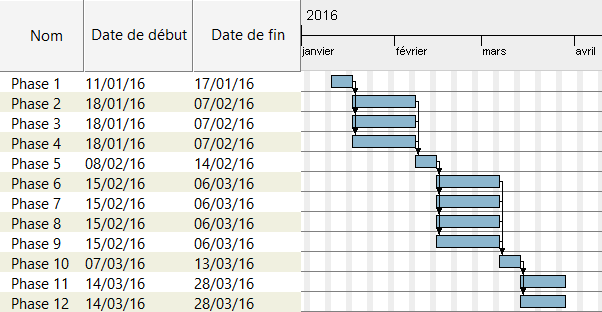
\includegraphics[scale=0.7]{gantt}
\caption{Diagramme de GANTT du projet}
\label{fig:gantt}
\end{figure}

\section{Fonctionnement}


Le déroulement de ce projet sera fait en mode supervisé, un rendez-vous hebdomadaire aura lieu à l’INRIA chaque mercredi hors vacances. 
Un rendez-vous avec le responsable pédagogique aura également lieu chaque semaine, le lundi.
Le cahier des charges est voué à être modifié au cours de l’étude car le développement peut amener à prendre en compte de nouvelles données qui créeront de nouveaux besoins en terme de démonstrations. 
L’application ne reposant pas sur un enjeu économique, des modifications - même importantes - ne seront pas vues comme un problème mais, au contraire, comme une opportunité d’amélioration et d’apprentissage.
Toute modification, ainsi que sa cause, seront répertoriées dans un carnet de bord et présentées dans un rapport final (qui présentera lui l’application « réelle », aboutissement du PFA, et les raisons des différences avec l’application initialement décrite dans ce cahier des charges). 
Une deuxième version de la documentation des bibliothèques et des API sera également créée car le développement de l’application améliorera notre connaissance et notre expertise sur ces dernières.

\section{Livrable}

En plus des rendez-vous hebdomadaires au cours duquel sera présenté l'avancement de chaque groupe, un rendu intermédiaire aura lieu en fin de phase 5, le livrable contiendra des fonctions codés en python permettant d'effectuer des regroupements de tweets à l'aide de machine learning et les résultats de l'analyse réalisés sur cette première partie.

En fin de PFA une application plus développé sera livré en fin de phase 10, cette application permettra d'effectuer le traitement complet des tweets présentées dans ce cahier des charges. Si le temps le permet, une version en ligne de l'application sera également livrée.



\end{document}